$\Ab\in\RR^{I_1I_2I_3\times J_1J_2J_3}$
(given as a TT-matrix) and a vector $\vb\in\RR^{I_1I_2I_3}$
(given in TT format) can be efficiently computed:
\begin{align}\label{eq:tt-mat-vec}
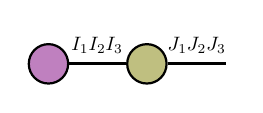
\begin{tikzpicture}[baseline=-0.5ex]
    \tikzset{tensor/.style = {minimum size = 0.5cm,shape = circle,thick,draw=black,inner sep = 0pt}, edge/.style = {thick,line width=.4mm},every loop/.style={}}
    \def\x{0}
    \def\y{0}
     \node[tensor,fill=green!50!red!50!white] (B) at (\x+1,\y) {$\Ab$};
    \node[tensor,fill=blue!50!red!50!white] (a) at (\x-0.25,\y) {$\vb$};
    \draw[edge] (B) -- (\x,\y) node [midway,above] {\scalebox{0.7}{\dimcolor{$I_1I_2I_3$}}};
    \draw[edge] (B) -- (\x+2,\y) node [midway,above] {\scalebox{0.7}{\dimcolor{$J_1J_2J_3$}}};
\end{tikzpicture}
=
\begin{tikzpicture}[baseline=\baseline]
    \tikzset{tensor/.style = {minimum size = 0.5cm,shape = circle,thick,draw=black,inner sep = 0pt}, edge/.style   = {thick,line width=.4mm},every loop/.style={}}
    \def\y{0}
    \def\x{0}
    \node[tensor,fill=red!30!white] (D) at (\x-1.5,\y){$\At_1$};
    \node[tensor,fill=red!50!white] (A) at (\x,\y){$\At_2$};
  \node[tensor,fill=blue!50!white] (B) at (\x+1.5,\y){$\At_3$};
    \draw[edge](A) -- (\x,\y-0.7)node [midway,left] {\edgelabel{$I_2$}};
    \draw[edge](B) -- (\x+1.5,\y-0.7)node [midway,left] {\edgelabel{$I_3$}};
     \draw[edge](D) -- (\x-1.5,\y-0.7)node [midway,left] {\edgelabel{$I_1$}};
    \draw[edge](D) -- (A) node [midway,above] {\edgelabel{$R_1$}};
    \draw[edge](A) -- (B) node [midway,above] {\edgelabel{$R_2$}};
    \draw[edge](A) -- (\x,\y+0.7)node [midway,left] {\edgelabel{$J_2$}};
    \draw[edge](B) -- (\x+1.5,\y+0.7)node [midway,left] {\edgelabel{$J_3$}};
    \draw[edge](D) -- (\x-1.5,\y+0.7)node [midway,left] {\edgelabel{$J_1$}};
    \node[tensor,fill=red!70!blue!40!white] (G1) at (\x-1.5,\y-0.9){$\Gt_1$};
    \node[tensor,fill=red!30!blue!30!white] (G2) at (\x,\y-0.9){$\Gt_2$};
  \node[tensor,fill=red!50!blue!50!white] (G3) at (\x+1.5,\y-0.9){$\Gt_3$};
  \draw[edge] (G1) -- (G2) node [midway,above] {\edgelabel{$S_1$}};
    \draw[edge] (G2) -- (G3) node [midway,above] {\edgelabel{$S_2$}};
\end{tikzpicture}
=~
\begin{tikzpicture}[baseline=\baseline]
    \tikzset{tensor/.style = {minimum size = 0.5cm,shape = circle,thick,draw=black,inner sep = 0pt}, edge/.style   = {thick,line width=.4mm},every loop/.style={}}
    \def\y{0}
    \def\x{0}
    \node[tensor,fill=cyan] (H1) at (\x-1.5,\y){$\Ht_1$};
    \node[tensor,fill=cyan!50!] (H2) at (\x,\y){$\Ht_2$};
   \node[tensor,fill=cyan!20!] (H3) at (\x+1.5,\y){$\Ht_3$};
   \draw[edge] (H1) -- (H2) node [midway,above]{\edgelabel{$R_1S_1$}};
    \draw[edge] (H2) -- (H3) node [midway,above]{\edgelabel{$R_2S_2$}};
    \draw[edge](H1) -- (\x-1.5,\y-0.7) node [midway, left]{\edgelabel{$J_1$}};
    \draw[edge](H2) -- (\x,\y-0.7)node [midway, left]{\edgelabel{$J_2$}};
    \draw[edge](H3) -- (\x+1.5,\y-0.7)node [midway, left]{\edgelabel{$J_3$}};
\end{tikzpicture}.
\end{align}
In the last equality, each pair of cores $\At_i,\Gt_i$ has been merged to obtain the core $\Ht_i$~(for $i = 1,2,3$), resulting in a  TT vector with ranks $(R_1 S_1, R_2 S_2)$. More generally, for an $N$-th order tensor, if $I_1 = \cdots = I_N = I$, $J_1 = \cdots = J_N = J$, $R_1 = \cdots = R_{N-1} = R$, and $S_1 = \cdots = S_{N-1} = S$, the overall computational complexity of the matrix-vector product is $\mathcal{O}(N R^2 S^2 I J)$.

As illustrated with the matrix-vector product above, performing operations in the TT format can lead to an increase in TT ranks. This applies to basic linear algebra operations, such as summation and the entry-wise product of
tensors. Although the resulting tensors remain in the TT format, the ranks typically grow as a consequence of these operations~\citep{oseledets2010approximation}. A summary of these operations and their effects on the TT ranks is provided in Table~\ref{tab:tt-operations}~\citep{novikov2014putting}. 
\begin{table}
\centering
\begin{tabular}{lll}
\toprule
\textsc{Operation} & \textsc{Output Ranks} & \textsc{Complexity} \\
\midrule
$\Ct = \At \cdot \text{const}$ & $R(\Ct) = R(\At)$ & $\mathcal{O}(d\,R(\At))$ \\
$\Ct = \At + \text{const}$ & $R(\Ct) \leq R(\At) + 1$ & $\mathcal{O}(nd\,R(\At)^2)$ \\
$\Ct = \At + \Bt$ & $R(\Ct) \leq R(\At) + R(\Bt)$ & $\mathcal{O}(nd\,R(\Ct)^2)$ \\
$\Ct = \At \krao \Bt$ & $R(\Ct) \leq R(\At)\,R(\Bt)$ & $\mathcal{O}(nd\,R(\At)^2\,R(\Bt)^2)$ \\
$\mathrm{sum} \At$ & -- & $\mathcal{O}(nd\,R(\At)^2)$ \\
$\norm{\At}_F$ & -- & $\mathcal{O}(nd\,R(\mathbf{A})^3)$ \\
\bottomrule
\end{tabular}
\caption{ Efficient operations on tensors in the TT-format~(table taken from~\citep{novikov2014putting}.)}
\label{tab:tt-operations}
\end{table}
In this table, the term $R$ refers to the maximal TT rank, i.e., $R(\At) = \max_{i=0,\dots,N} R_i$, $n$ to the order of the tensor, and $d$ to its maximal dimension.

The TT-rounding algorithm~\citep{oseledets2010approximation} can be used to reduce the ranks when needed~(at the cost of some approximation error). 

\paragraph{TT-rounding} As noted earlier, tensor operations in the TT format, such as addition or multiplication, generally lead to an increase in the TT ranks. To prevent uncontrolled rank growth while maintaining accuracy, it is necessary to perform rank reduction. This is achieved by applying a \emph{TT-rounding} procedure: starting from an $N$-th order TT tensor with ranks $R^\prime_k$ for $k\in[N-1]$, the goal is to find a good approximation with lower TT rank $R_k$. A naive and inefficient way to achieve this would be to reconstruct the full tensor and perform TT-SVD to obtain a rank $(R_1,\cdots,R_{N-1})$ TT approximation. It turns out that this can be done without reconstructing the full tensor! We show that the following procedure is exactly equivalent to performing TT-SVD on the full tensor.

First, the tensor is orthogonalized by performing a sequence of QR decompositions on the TT cores in a left-to-right (or right-to-left) sweep. Subsequently, a truncation step is performed on each core using a truncated SVD, where singular values are discarded according to a prescribed rank-$R_k$. The truncated factors are then redistributed back into adjacent TT cores, yielding a new TT representation with reduced ranks while controlling the approximation error. As an illustrative example, let us consider a fourth-order tensor given in the TT format with rank-$R^\prime_k$. As a first step, we perform the QR decomposition from right to left:
\begin{align*}
&\begin{tikzpicture}[baseline=\baseline]
    \tikzset{tensor/.style = {minimum size = 0.5cm,shape = circle,thick,draw=black,inner sep = 0pt}, edge/.style   = {thick,line width=.4mm},every loop/.style={}}
    \def\y{0}
    \def\x{0}
    \node[tensor,fill=cyan] (G1) at (\x-3,\y){$\Gt_1$};
    \node[tensor,fill=cyan!60!] (G2) at (\x-2,\y){$\Gt_2$};
    \node[tensor,fill=cyan!40!] (G3) at (\x-1,\y){$\Gt_3$};
   \node[tensor,fill=cyan!20!] (G4) at (\x,\y){$\Gt_4$};
   \draw[edge] (G1) -- (G2) node [midway,above]{\edgelabel{$R^\prime_1$}};
    \draw[edge] (G2) -- (G3) node [midway,above]{\edgelabel{$R^\prime_2$}};
    \draw[edge] (G3) -- (G4) node [midway,above]{\edgelabel{$R^\prime_3$}};
    \draw[edge](G1) -- (\x-3,\y-0.7) node [midway, left]{\edgelabel{$d_1$}};
    \draw[edge](G2) -- (\x-2,\y-0.7)node [midway, left]{\edgelabel{$d_2$}};
    \draw[edge](G3) -- (\x-1,\y-0.7)node [midway, left]{\edgelabel{$d_3$}};
    \draw[edge](G4) -- (\x,\y-0.7)node [midway, left]{\edgelabel{$d_4$}};
    \node[draw=none] at (\x+3.5,\y){$\underrightarrow{\text{QR decomposition from right to left}}$};
\end{tikzpicture}
\begin{tikzpicture}[baseline=\baseline]
    \tikzset{tensor/.style = {minimum size = 0.5cm,shape = circle,thick,draw=black,inner sep = 0pt}, edge/.style = {thick,line width=.4mm},every loop/.style={}}
    \def\y{0}
    \def\x{0}
        \node[tensor,fill=cyan] (G1) at (\x-3,\y){$\Gt_1$};
    \node[tensor,fill=cyan!60!] (G2) at (\x-2,\y){$\Gt_2$};
    \node[tensor,fill=cyan!40!] (G3) at (\x-1,\y){$\Gt_3$};
    \node[tensor, path picture={
    \fill[fill=cyan!20!](path picture bounding box.south west)
    -- 
    (path picture bounding box.north east) --
    (path picture bounding box.north west) -- cycle;}, shift={(\x+1,\y)}] (G4) {$\Qt_4$};
    \node[tensor,fill=cyan!20!] (R4) at (\x,\y){$\Rb_4$};
   \draw[edge] (G1) -- (G2) node [midway,above]{\edgelabel{$R^\prime_1$}};
    \draw[edge] (G2) -- (G3) node [midway,above]{\edgelabel{$R^\prime_2$}};
    \draw[edge] (G3) -- (R4) node [midway,above]{\edgelabel{$R^\prime_3$}};
    \draw[edge] (R4) -- (G4) node [midway,above]{\edgelabel{$R^\prime_3$}};
    \draw[edge](G1) -- (\x-3,\y-0.7) node [midway, left]{\edgelabel{$d_1$}};
    \draw[edge](G2) -- (\x-2,\y-0.7)node [midway, left]{\edgelabel{$d_2$}};
    \draw[edge](G3) -- (\x-1,\y-0.7)node [midway, left]{\edgelabel{$d_3$}};
    \draw[edge](G4) -- (\x+1,\y-0.7)node [midway,left] {\scalebox{0.7}{\dimcolor{$d_4$}}};
    \node[draw=none] at (\x-0.5,\y+0.7){$\overbrace{\hspace{1cm}}^{\text{merge \& apply QR}}$};
    \end{tikzpicture}\\
&\begin{tikzpicture}[baseline=\baseline]
    \tikzset{tensor/.style = {minimum size = 0.5cm,shape = circle,thick,draw=black,inner sep = 0pt}, edge/.style = {thick,line width=.4mm},every loop/.style={}}
    \def\y{0}
    \def\x{0}
        \node[tensor,fill=cyan] (G1) at (\x-3,\y){$\Gt_1$};
    \node[tensor,fill=cyan!60!] (G2) at (\x-2,\y){$\Gt_2$};
    \node[tensor, path picture={
    \fill[fill=cyan!40!](path picture bounding box.south west)
    -- 
    (path picture bounding box.north east) --
    (path picture bounding box.north west) -- cycle;}, shift={(\x,\y)}] (G3) {$\Qt_3$};
    \node[tensor, path picture={
    \fill[fill=cyan!20!](path picture bounding box.south west)
    -- 
    (path picture bounding box.north east) --
    (path picture bounding box.north west) -- cycle;}, shift={(\x+1,\y)}] (G4) {$\Qt_4$};
    \node[tensor,fill=cyan!40!] (R3) at (\x-1,\y){$\Rb_3$};
   \draw[edge] (G1) -- (G2) node [midway,above]{\edgelabel{$R^\prime_1$}};
    \draw[edge] (G2) -- (R3) node [midway,above]{\edgelabel{$R^\prime_2$}};
    \draw[edge] (R3) -- (G3) node [midway,above]{\edgelabel{$R^\prime_3$}};
    \draw[edge] (G3) -- (G4) node [midway,above]{\edgelabel{$R^\prime_3$}};
    \draw[edge](G1) -- (\x-3,\y-0.7) node [midway, left]{\edgelabel{$d_1$}};
    \draw[edge](G2) -- (\x-2,\y-0.7)node [midway, left]{\edgelabel{$d_2$}};
    \draw[edge](G3) -- (\x,\y-0.7)node [midway, left]{\edgelabel{$d_3$}};
    \draw[edge](G4) -- (\x+1,\y-0.7)node [midway,left] {\scalebox{0.7}{\dimcolor{$d_4$}}};
    \node[draw=none] at (\x-1.5,\y+0.7){$\overbrace{\hspace{1cm}}^{\text{merge \& apply QR}}$};
    \node[draw=none] at (\x+2,\y){$\cdots$};
    \end{tikzpicture}
\begin{tikzpicture}[baseline=\baseline]
    \tikzset{tensor/.style = {minimum size = 0.5cm,shape = circle,thick,draw=black,inner sep = 0pt}, edge/.style = {thick,line width=.4mm},every loop/.style={}}
    \def\y{0}
    \def\x{0}
    \node[tensor,fill=cyan] (G1) at (\x-3,\y){$\Tilde{\Gt_1}$};
    \node[tensor, path picture={
    \fill[fill=cyan!60!](path picture bounding box.south west)
    -- 
    (path picture bounding box.north east) --
    (path picture bounding box.north west) -- cycle;}, shift={(\x-2,\y)}] (G2) {$\Qt_2$};
    \node[tensor, path picture={
    \fill[fill=cyan!40!](path picture bounding box.south west)
    -- 
    (path picture bounding box.north east) --
    (path picture bounding box.north west) -- cycle;}, shift={(\x-1,\y)}] (G3) {$\Qt_3$};
    \node[tensor, path picture={
    \fill[fill=cyan!20!](path picture bounding box.south west)
    -- 
    (path picture bounding box.north east) --
    (path picture bounding box.north west) -- cycle;}, shift={(\x,\y)}] (G4) {$\Qt_4$};
   \draw[edge] (G1) -- (G2) node [midway,above]{\edgelabel{$R^\prime_1$}};
      \draw[edge] (G2) -- (G3) node [midway,above]{\edgelabel{$R^\prime_2$}};
    \draw[edge] (G3) -- (G4) node [midway,above]{\edgelabel{$R^\prime_3$}};
    \draw[edge](G1) -- (\x-3,\y-0.7) node [midway, left]{\edgelabel{$d_1$}};
    \draw[edge](G2) -- (\x-2,\y-0.7)node [midway, left]{\edgelabel{$d_2$}};
    \draw[edge](G3) -- (\x-1,\y-0.7)node [midway, left]{\edgelabel{$d_3$}};
    \draw[edge](G4) -- (\x,\y-0.7)node [midway,left] {\scalebox{0.7}{\dimcolor{$d_4$}}};
    \end{tikzpicture}.
\end{align*}
The procedure continues with truncated SVDs from left to right:
\begin{align*}
&\begin{tikzpicture}[baseline=\baseline]
    \tikzset{tensor/.style = {minimum size = 0.5cm,shape = circle,thick,draw=black,inner sep = 0pt}, edge/.style = {thick,line width=.4mm},every loop/.style={}}
    \def\x{0}
    \def\y{0}
    \node[tensor,fill=cyan] (G1) at (\x-3,\y){$\Tilde{\Gt_1}$};
    \node[tensor, path picture={
    \fill[fill=cyan!60!](path picture bounding box.south west)
    -- 
    (path picture bounding box.north east) --
    (path picture bounding box.north west) -- cycle;}, shift={(\x-2,\y)}] (G2) {$\Qt_2$};
    \node[tensor, path picture={
    \fill[fill=cyan!40!](path picture bounding box.south west)
    -- 
    (path picture bounding box.north east) --
    (path picture bounding box.north west) -- cycle;}, shift={(\x-1,\y)}] (G3) {$\Qt_3$};
    \node[tensor, path picture={
    \fill[fill=cyan!20!](path picture bounding box.south west)
    -- 
    (path picture bounding box.north east) --
    (path picture bounding box.north west) -- cycle;}, shift={(\x,\y)}] (G4) {$\Qt_4$};
   \draw[edge] (G1) -- (G2) node [midway,above]{\edgelabel{$R^\prime_1$}};
      \draw[edge] (G2) -- (G3) node [midway,above]{\edgelabel{$R^\prime_2$}};
    \draw[edge] (G3) -- (G4) node [midway,above]{\edgelabel{$R^\prime_3$}};
    \draw[edge](G1) -- (\x-3,\y-0.7) node [midway, left]{\edgelabel{$d_1$}};
    \draw[edge](G2) -- (\x-2,\y-0.7)node [midway, left]{\edgelabel{$d_2$}};
    \draw[edge](G3) -- (\x-1,\y-0.7)node [midway, left]{\edgelabel{$d_3$}};
    \draw[edge](G4) -- (\x,\y-0.7)node [midway,left] {\scalebox{0.7}{\dimcolor{$d_4$}}};
    \node[draw=none] at (\x+3.25,\y){$\underrightarrow{\text{rank-$R_1$ truncated SVD of $\tilde \Gt_1$}}$};
    \end{tikzpicture}
\begin{tikzpicture}[baseline=\baseline]
    \tikzset{tensor/.style = {minimum size = 0.5cm,shape = circle,thick,draw=black,inner sep = 0pt}, edge/.style = {thick,line width=.4mm},every loop/.style={}}
    \def\y{0}
    \def\x{0}
     \node[tensor, path picture={
    \fill[fill=cyan](path picture bounding box.south east)
    -- 
    (path picture bounding box.north west) --
    (path picture bounding box.north east) -- cycle;}, shift={(\x-3,\y)}] (U1) {$\Gt_1$};
    \node[tensor,fill=cyan] (sigma) at (\x-2,\y){{}};
    \draw[edge=0.5] (sigma.south west) -- (sigma.north        east);
    \node[tensor, path picture={
    \fill[fill=cyan](path picture bounding box.south west)
    -- 
    (path picture bounding box.north east) --
    (path picture bounding box.north west) -- cycle;}, shift={(\x-1,\y)}] (V1) {$\Vb_1$};
    \node[tensor, path picture={
    \fill[fill=cyan!60!](path picture bounding box.south west)
    -- 
    (path picture bounding box.north east) --
    (path picture bounding box.north west) -- cycle;}, shift={(\x,\y)}] (G2) {$\Qt_2$};
    \node[tensor, path picture={
    \fill[fill=cyan!40!](path picture bounding box.south west)
    -- 
    (path picture bounding box.north east) --
    (path picture bounding box.north west) -- cycle;}, shift={(\x+1,\y)}] (G3) {$\Qt_3$};
    \node[tensor, path picture={
    \fill[fill=cyan!20!](path picture bounding box.south west)
    -- 
    (path picture bounding box.north east) --
    (path picture bounding box.north west) -- cycle;}, shift={(\x+2,\y)}] (G4) {$\Qt_4$};
   \draw[edge] (U1) -- (sigma) node [midway,above]{\edgelabel{$R_1$}};
      \draw[edge] (sigma) -- (V1) node [midway,above]{\edgelabel{$R_1$}};
    \draw[edge] (V1) -- (G2) node [midway,above]{\edgelabel{$R_1$}};
    \draw[edge] (G2) -- (G3) node [midway,above]{\edgelabel{$R^\prime_2$}};
    \draw[edge] (G3) -- (G4) node [midway,above]{\edgelabel{$R^\prime_3$}};
    \draw[edge](U1) -- (\x-3,\y-0.7) node [midway, left]{\edgelabel{$d_1$}};
    \draw[edge](G2) -- (\x,\y-0.7)node [midway, left]{\edgelabel{$d_2$}};
    \draw[edge](G3) -- (\x+1,\y-0.7)node [midway, left]{\edgelabel{$d_3$}};
    \draw[edge](G4) -- (\x+2,\y-0.7)node [midway,left] {\scalebox{0.7}{\dimcolor{$d_4$}}};
    \node[draw=none] at (\x-1,\y+0.7){$\overbrace{\hspace{2cm}}^{\text{merge \& apply rank-$R_2$ SVD}}$};
    \end{tikzpicture}\\
&\begin{tikzpicture}[baseline=\baseline]
    \tikzset{tensor/.style = {minimum size = 0.5cm,shape = circle,thick,draw=black,inner sep = 0pt}, edge/.style = {thick,line width=.4mm},every loop/.style={}}
    \def\y{0}
    \def\x{0}
     \node[tensor, path picture={
    \fill[fill=cyan](path picture bounding box.south east)
    -- 
    (path picture bounding box.north west) --
    (path picture bounding box.north east) -- cycle;}, shift={(\x-3,\y)}] (U1) {$\Gt_1$};
    \node[tensor, path picture={
    \fill[fill=cyan!60!](path picture bounding box.south east)
    -- 
    (path picture bounding box.north west) --
    (path picture bounding box.north east) -- cycle;}, shift={(\x-2,\y)}] (G2) {$\Gt_2$};
    \node[tensor,fill=cyan!60!] (sigma) at (\x-1,\y){{}};
    \draw[edge=0.5] (sigma.south west) -- (sigma.north        east);
    \node[tensor, path picture={
    \fill[fill=cyan!60!](path picture bounding box.south west)
    -- 
    (path picture bounding box.north east) --
    (path picture bounding box.north west) -- cycle;}, shift={(\x,\y)}] (V2) {$\Vb_2$};
    \node[tensor, path picture={
    \fill[fill=cyan!40!](path picture bounding box.south west)
    -- 
    (path picture bounding box.north east) --
    (path picture bounding box.north west) -- cycle;}, shift={(\x+1,\y)}] (G3) {$\Qt_3$};
    \node[tensor, path picture={
    \fill[fill=cyan!20!](path picture bounding box.south west)
    -- 
    (path picture bounding box.north east) --
    (path picture bounding box.north west) -- cycle;}, shift={(\x+2,\y)}] (G4) {$\Qt_4$};
   \draw[edge] (U1) -- (G2) node [midway,above]{\edgelabel{$R_1$}};
      \draw[edge] (G2) -- (sigma) node [midway,above]{\edgelabel{$R_2$}};
    \draw[edge] (sigma) -- (V2) node [midway,above]{\edgelabel{$R_2$}};
    \draw[edge] (V2) -- (G3) node [midway,above]{\edgelabel{$R^\prime_2$}};
    \draw[edge] (G3) -- (G4) node [midway,above]{\edgelabel{$R^\prime_3$}};
    \draw[edge](U1) -- (\x-3,\y-0.7) node [midway, left]{\edgelabel{$d_1$}};
    \draw[edge](G2) -- (\x-2,\y-0.7)node [midway, left]{\edgelabel{$d_2$}};
    \draw[edge](G3) -- (\x+1,\y-0.7)node [midway, left]{\edgelabel{$d_3$}};
    \draw[edge](G4) -- (\x+2,\y-0.7)node [midway,left] {\scalebox{0.7}{\dimcolor{$d_4$}}};
    \node[draw=none] at (\x,\y+0.7){$\overbrace{\hspace{2cm}}^{\text{merge \& apply rank-$R_3$ SVD}}$};
    \node[draw=none] at (\x+3,\y){$\longrightarrow$};
    \end{tikzpicture}
\begin{tikzpicture}[baseline=\baseline]
    \tikzset{tensor/.style = {minimum size = 0.5cm,shape = circle,thick,draw=black,inner sep = 0pt}, edge/.style = {thick,line width=.4mm},every loop/.style={}}
    \def\y{0}
    \def\x{0}
     \node[tensor, path picture={
    \fill[fill=cyan](path picture bounding box.south east)
    -- 
    (path picture bounding box.north west) --
    (path picture bounding box.north east) -- cycle;}, shift={(\x-3,\y)}] (U1) {$\Gt_1$};
    \node[tensor, path picture={
    \fill[fill=cyan!60!](path picture bounding box.south east)
    -- 
    (path picture bounding box.north west) --
    (path picture bounding box.north east) -- cycle;}, shift={(\x-2,\y)}] (G2) {$\Gt_2$};
    \node[tensor, path picture={
    \fill[fill=cyan!40!](path picture bounding box.south east)
    -- 
    (path picture bounding box.north west) --
    (path picture bounding box.north east) -- cycle;}, shift={(\x-1,\y)}] (G3) {$\Gt_3$};
    \node[tensor,fill=cyan!40!] (sigma) at (\x,\y){{}};
    \draw[edge=0.5] (sigma.south west) -- (sigma.north        east);
    \node[tensor, path picture={
    \fill[fill=cyan!40!](path picture bounding box.south west)
    -- 
    (path picture bounding box.north east) --
    (path picture bounding box.north west) -- cycle;}, shift={(\x+1,\y)}] (V3) {$\Vb_3$};
    \node[tensor, path picture={
    \fill[fill=cyan!20!](path picture bounding box.south west)
    -- 
    (path picture bounding box.north east) --
    (path picture bounding box.north west) -- cycle;}, shift={(\x+2,\y)}] (G4) {$\Qt_4$};
   \draw[edge] (U1) -- (G2) node [midway,above]{\edgelabel{$R_1$}};
      \draw[edge] (G2) -- (G3) node [midway,above]{\edgelabel{$R_2$}};
    \draw[edge] (G3) -- (sigma) node [midway,above]{\edgelabel{$R_3$}};
    \draw[edge] (sigma) -- (V3) node [midway,above]{\edgelabel{$R_3$}};
    \draw[edge] (V3) -- (G4) node [midway,above]{\edgelabel{$R^\prime_3$}};
    \draw[edge](U1) -- (\x-3,\y-0.7) node [midway, left]{\edgelabel{$d_1$}};
    \draw[edge](G2) -- (\x-2,\y-0.7)node [midway, left]{\edgelabel{$d_2$}};
    \draw[edge](G3) -- (\x-1,\y-0.7)node [midway, left]{\edgelabel{$d_3$}};
    \draw[edge](G4) -- (\x+2,\y-0.7)node [midway,left] {\scalebox{0.7}{\dimcolor{$d_4$}}};
    \node[draw=none] at (\x+1,\y+0.7){$\overbrace{\hspace{2cm}}^{\text{merge}}$};
    \node[draw=none] at (\x+3,\y){$\longrightarrow$};
    \end{tikzpicture}\\
&\begin{tikzpicture}[baseline=\baseline]
    \tikzset{tensor/.style = {minimum size = 0.5cm,shape = circle,thick,draw=black,inner sep = 0pt}, edge/.style = {thick,line width=.4mm},every loop/.style={}}
    \def\y{0}
    \def\x{0}
     \node[tensor, path picture={
    \fill[fill=cyan](path picture bounding box.south east)
    -- 
    (path picture bounding box.north west) --
    (path picture bounding box.north east) -- cycle;}, shift={(\x-3,\y)}] (U1) {$\Gt_1$};
    \node[tensor, path picture={
    \fill[fill=cyan!60!](path picture bounding box.south east)
    -- 
    (path picture bounding box.north west) --
    (path picture bounding box.north east) -- cycle;}, shift={(\x-2,\y)}] (G2) {$\Gt_2$};
    \node[tensor, path picture={
    \fill[fill=cyan!40!](path picture bounding box.south east)
    -- 
    (path picture bounding box.north west) --
    (path picture bounding box.north east) -- cycle;}, shift={(\x-1,\y)}] (G3) {$\Gt_3$};
    \node[tensor,fill=cyan!20!] (G4) at (\x,\y){$\Gt_4$};
   \draw[edge] (U1) -- (G2) node [midway,above]{\edgelabel{$R_1$}};
      \draw[edge] (G2) -- (G3) node [midway,above]{\edgelabel{$R_2$}};
    \draw[edge] (G3) -- (G4) node [midway,above]{\edgelabel{$R_3$}};
    \draw[edge](U1) -- (\x-3,\y-0.7) node [midway, left]{\edgelabel{$d_1$}};
    \draw[edge](G2) -- (\x-2,\y-0.7)node [midway, left]{\edgelabel{$d_2$}};
    \draw[edge](G3) -- (\x-1,\y-0.7)node [midway, left]{\edgelabel{$d_3$}};
    \draw[edge](G4) -- (\x,\y-0.7)node [midway,left] {\scalebox{0.7}{\dimcolor{$d_4$}}};
    \end{tikzpicture},   
\end{align*}
